% Options for packages loaded elsewhere
\PassOptionsToPackage{unicode}{hyperref}
\PassOptionsToPackage{hyphens}{url}
\PassOptionsToPackage{dvipsnames,svgnames,x11names}{xcolor}
%
\documentclass[
  letterpaper,
  DIV=11,
  numbers=noendperiod]{scrartcl}

\usepackage{amsmath,amssymb}
\usepackage{iftex}
\ifPDFTeX
  \usepackage[T1]{fontenc}
  \usepackage[utf8]{inputenc}
  \usepackage{textcomp} % provide euro and other symbols
\else % if luatex or xetex
  \usepackage{unicode-math}
  \defaultfontfeatures{Scale=MatchLowercase}
  \defaultfontfeatures[\rmfamily]{Ligatures=TeX,Scale=1}
\fi
\usepackage{lmodern}
\ifPDFTeX\else  
    % xetex/luatex font selection
\fi
% Use upquote if available, for straight quotes in verbatim environments
\IfFileExists{upquote.sty}{\usepackage{upquote}}{}
\IfFileExists{microtype.sty}{% use microtype if available
  \usepackage[]{microtype}
  \UseMicrotypeSet[protrusion]{basicmath} % disable protrusion for tt fonts
}{}
\makeatletter
\@ifundefined{KOMAClassName}{% if non-KOMA class
  \IfFileExists{parskip.sty}{%
    \usepackage{parskip}
  }{% else
    \setlength{\parindent}{0pt}
    \setlength{\parskip}{6pt plus 2pt minus 1pt}}
}{% if KOMA class
  \KOMAoptions{parskip=half}}
\makeatother
\usepackage{xcolor}
\setlength{\emergencystretch}{3em} % prevent overfull lines
\setcounter{secnumdepth}{-\maxdimen} % remove section numbering
% Make \paragraph and \subparagraph free-standing
\ifx\paragraph\undefined\else
  \let\oldparagraph\paragraph
  \renewcommand{\paragraph}[1]{\oldparagraph{#1}\mbox{}}
\fi
\ifx\subparagraph\undefined\else
  \let\oldsubparagraph\subparagraph
  \renewcommand{\subparagraph}[1]{\oldsubparagraph{#1}\mbox{}}
\fi

\usepackage{color}
\usepackage{fancyvrb}
\newcommand{\VerbBar}{|}
\newcommand{\VERB}{\Verb[commandchars=\\\{\}]}
\DefineVerbatimEnvironment{Highlighting}{Verbatim}{commandchars=\\\{\}}
% Add ',fontsize=\small' for more characters per line
\usepackage{framed}
\definecolor{shadecolor}{RGB}{241,243,245}
\newenvironment{Shaded}{\begin{snugshade}}{\end{snugshade}}
\newcommand{\AlertTok}[1]{\textcolor[rgb]{0.68,0.00,0.00}{#1}}
\newcommand{\AnnotationTok}[1]{\textcolor[rgb]{0.37,0.37,0.37}{#1}}
\newcommand{\AttributeTok}[1]{\textcolor[rgb]{0.40,0.45,0.13}{#1}}
\newcommand{\BaseNTok}[1]{\textcolor[rgb]{0.68,0.00,0.00}{#1}}
\newcommand{\BuiltInTok}[1]{\textcolor[rgb]{0.00,0.23,0.31}{#1}}
\newcommand{\CharTok}[1]{\textcolor[rgb]{0.13,0.47,0.30}{#1}}
\newcommand{\CommentTok}[1]{\textcolor[rgb]{0.37,0.37,0.37}{#1}}
\newcommand{\CommentVarTok}[1]{\textcolor[rgb]{0.37,0.37,0.37}{\textit{#1}}}
\newcommand{\ConstantTok}[1]{\textcolor[rgb]{0.56,0.35,0.01}{#1}}
\newcommand{\ControlFlowTok}[1]{\textcolor[rgb]{0.00,0.23,0.31}{#1}}
\newcommand{\DataTypeTok}[1]{\textcolor[rgb]{0.68,0.00,0.00}{#1}}
\newcommand{\DecValTok}[1]{\textcolor[rgb]{0.68,0.00,0.00}{#1}}
\newcommand{\DocumentationTok}[1]{\textcolor[rgb]{0.37,0.37,0.37}{\textit{#1}}}
\newcommand{\ErrorTok}[1]{\textcolor[rgb]{0.68,0.00,0.00}{#1}}
\newcommand{\ExtensionTok}[1]{\textcolor[rgb]{0.00,0.23,0.31}{#1}}
\newcommand{\FloatTok}[1]{\textcolor[rgb]{0.68,0.00,0.00}{#1}}
\newcommand{\FunctionTok}[1]{\textcolor[rgb]{0.28,0.35,0.67}{#1}}
\newcommand{\ImportTok}[1]{\textcolor[rgb]{0.00,0.46,0.62}{#1}}
\newcommand{\InformationTok}[1]{\textcolor[rgb]{0.37,0.37,0.37}{#1}}
\newcommand{\KeywordTok}[1]{\textcolor[rgb]{0.00,0.23,0.31}{#1}}
\newcommand{\NormalTok}[1]{\textcolor[rgb]{0.00,0.23,0.31}{#1}}
\newcommand{\OperatorTok}[1]{\textcolor[rgb]{0.37,0.37,0.37}{#1}}
\newcommand{\OtherTok}[1]{\textcolor[rgb]{0.00,0.23,0.31}{#1}}
\newcommand{\PreprocessorTok}[1]{\textcolor[rgb]{0.68,0.00,0.00}{#1}}
\newcommand{\RegionMarkerTok}[1]{\textcolor[rgb]{0.00,0.23,0.31}{#1}}
\newcommand{\SpecialCharTok}[1]{\textcolor[rgb]{0.37,0.37,0.37}{#1}}
\newcommand{\SpecialStringTok}[1]{\textcolor[rgb]{0.13,0.47,0.30}{#1}}
\newcommand{\StringTok}[1]{\textcolor[rgb]{0.13,0.47,0.30}{#1}}
\newcommand{\VariableTok}[1]{\textcolor[rgb]{0.07,0.07,0.07}{#1}}
\newcommand{\VerbatimStringTok}[1]{\textcolor[rgb]{0.13,0.47,0.30}{#1}}
\newcommand{\WarningTok}[1]{\textcolor[rgb]{0.37,0.37,0.37}{\textit{#1}}}

\providecommand{\tightlist}{%
  \setlength{\itemsep}{0pt}\setlength{\parskip}{0pt}}\usepackage{longtable,booktabs,array}
\usepackage{calc} % for calculating minipage widths
% Correct order of tables after \paragraph or \subparagraph
\usepackage{etoolbox}
\makeatletter
\patchcmd\longtable{\par}{\if@noskipsec\mbox{}\fi\par}{}{}
\makeatother
% Allow footnotes in longtable head/foot
\IfFileExists{footnotehyper.sty}{\usepackage{footnotehyper}}{\usepackage{footnote}}
\makesavenoteenv{longtable}
\usepackage{graphicx}
\makeatletter
\def\maxwidth{\ifdim\Gin@nat@width>\linewidth\linewidth\else\Gin@nat@width\fi}
\def\maxheight{\ifdim\Gin@nat@height>\textheight\textheight\else\Gin@nat@height\fi}
\makeatother
% Scale images if necessary, so that they will not overflow the page
% margins by default, and it is still possible to overwrite the defaults
% using explicit options in \includegraphics[width, height, ...]{}
\setkeys{Gin}{width=\maxwidth,height=\maxheight,keepaspectratio}
% Set default figure placement to htbp
\makeatletter
\def\fps@figure{htbp}
\makeatother

\KOMAoption{captions}{tableheading}
\makeatletter
\makeatother
\makeatletter
\makeatother
\makeatletter
\@ifpackageloaded{caption}{}{\usepackage{caption}}
\AtBeginDocument{%
\ifdefined\contentsname
  \renewcommand*\contentsname{Table of contents}
\else
  \newcommand\contentsname{Table of contents}
\fi
\ifdefined\listfigurename
  \renewcommand*\listfigurename{List of Figures}
\else
  \newcommand\listfigurename{List of Figures}
\fi
\ifdefined\listtablename
  \renewcommand*\listtablename{List of Tables}
\else
  \newcommand\listtablename{List of Tables}
\fi
\ifdefined\figurename
  \renewcommand*\figurename{Figure}
\else
  \newcommand\figurename{Figure}
\fi
\ifdefined\tablename
  \renewcommand*\tablename{Table}
\else
  \newcommand\tablename{Table}
\fi
}
\@ifpackageloaded{float}{}{\usepackage{float}}
\floatstyle{ruled}
\@ifundefined{c@chapter}{\newfloat{codelisting}{h}{lop}}{\newfloat{codelisting}{h}{lop}[chapter]}
\floatname{codelisting}{Listing}
\newcommand*\listoflistings{\listof{codelisting}{List of Listings}}
\makeatother
\makeatletter
\@ifpackageloaded{caption}{}{\usepackage{caption}}
\@ifpackageloaded{subcaption}{}{\usepackage{subcaption}}
\makeatother
\makeatletter
\@ifpackageloaded{tcolorbox}{}{\usepackage[skins,breakable]{tcolorbox}}
\makeatother
\makeatletter
\@ifundefined{shadecolor}{\definecolor{shadecolor}{rgb}{.97, .97, .97}}
\makeatother
\makeatletter
\makeatother
\makeatletter
\makeatother
\ifLuaTeX
  \usepackage{selnolig}  % disable illegal ligatures
\fi
\IfFileExists{bookmark.sty}{\usepackage{bookmark}}{\usepackage{hyperref}}
\IfFileExists{xurl.sty}{\usepackage{xurl}}{} % add URL line breaks if available
\urlstyle{same} % disable monospaced font for URLs
\hypersetup{
  pdftitle={Reproducible Research Project: Air Passengers Occupancy Prediction},
  pdfauthor={Adam Foster, Maciej Staniszewski, Illia Baranochnikov},
  colorlinks=true,
  linkcolor={blue},
  filecolor={Maroon},
  citecolor={Blue},
  urlcolor={Blue},
  pdfcreator={LaTeX via pandoc}}

\title{Reproducible Research Project: Air Passengers Occupancy
Prediction}
\author{Adam Foster, Maciej Staniszewski, Illia Baranochnikov}
\date{}

\begin{document}
\maketitle
\ifdefined\Shaded\renewenvironment{Shaded}{\begin{tcolorbox}[enhanced, boxrule=0pt, sharp corners, borderline west={3pt}{0pt}{shadecolor}, interior hidden, frame hidden, breakable]}{\end{tcolorbox}}\fi

\hypertarget{importing-libraries}{%
\section{Importing Libraries}\label{importing-libraries}}

\begin{Shaded}
\begin{Highlighting}[]
\ImportTok{import}\NormalTok{ pandas }\ImportTok{as}\NormalTok{ pd}
\ImportTok{import}\NormalTok{ matplotlib.pyplot }\ImportTok{as}\NormalTok{ plt}
\ImportTok{import}\NormalTok{ statsmodels.api }\ImportTok{as}\NormalTok{ sm}
\ImportTok{import}\NormalTok{ datetime}
\ImportTok{from}\NormalTok{ scipy.stats }\ImportTok{import}\NormalTok{ norm}
\ImportTok{from}\NormalTok{ statsmodels.tsa.arima.model }\ImportTok{import}\NormalTok{ ARIMA}
\ImportTok{from}\NormalTok{ statsmodels.tsa.seasonal }\ImportTok{import}\NormalTok{ seasonal\_decompose}
\ImportTok{from}\NormalTok{ sklearn.metrics }\ImportTok{import}\NormalTok{ mean\_squared\_error}
\end{Highlighting}
\end{Shaded}

\hypertarget{loading-the-dataset}{%
\section{Loading the Dataset}\label{loading-the-dataset}}

Air passenger data is downloaded to the \texttt{/data} subdirectory of
the root project folder. We will use \texttt{pandas} to create a data
frame with this data.

\begin{Shaded}
\begin{Highlighting}[]
\NormalTok{data }\OperatorTok{=}\NormalTok{ pd.read\_csv(}\StringTok{\textquotesingle{}data/AirPassengers.xls\textquotesingle{}}\NormalTok{, index\_col}\OperatorTok{=}\DecValTok{0}\NormalTok{)}
\NormalTok{data.columns }\OperatorTok{=}\NormalTok{ [ }\StringTok{\textquotesingle{}Count\textquotesingle{}}\NormalTok{ ] }\CommentTok{\# Renaming \textasciigrave{}\#Passengers\textasciigrave{} {-}\textgreater{} \textasciigrave{}Count\textasciigrave{} for convenience}
\NormalTok{data.head()}
\end{Highlighting}
\end{Shaded}

\begin{longtable}[]{@{}ll@{}}
\toprule\noalign{}
& Count \\
Month & \\
\midrule\noalign{}
\endhead
\bottomrule\noalign{}
\endlastfoot
1949-01 & 112 \\
1949-02 & 118 \\
1949-03 & 132 \\
1949-04 & 129 \\
1949-05 & 121 \\
\end{longtable}

\begin{Shaded}
\begin{Highlighting}[]
\NormalTok{data.tail()}
\end{Highlighting}
\end{Shaded}

\begin{longtable}[]{@{}ll@{}}
\toprule\noalign{}
& Count \\
Month & \\
\midrule\noalign{}
\endhead
\bottomrule\noalign{}
\endlastfoot
1960-08 & 606 \\
1960-09 & 508 \\
1960-10 & 461 \\
1960-11 & 390 \\
1960-12 & 432 \\
\end{longtable}

We see that the dataset looks relatively simple. It contains monthly
data about the number of air passengers from 1949 to 1960. Let's see
more detailed description of the data using \texttt{pandas.describe()}:

\begin{Shaded}
\begin{Highlighting}[]
\NormalTok{data.describe()}
\end{Highlighting}
\end{Shaded}

\begin{longtable}[]{@{}ll@{}}
\toprule\noalign{}
& Count \\
\midrule\noalign{}
\endhead
\bottomrule\noalign{}
\endlastfoot
count & 144.000000 \\
mean & 280.298611 \\
std & 119.966317 \\
min & 104.000000 \\
25\% & 180.000000 \\
50\% & 265.500000 \\
75\% & 360.500000 \\
max & 622.000000 \\
\end{longtable}

Having taken a better look we can note down a couple observations: -
There are 144 observations - The distribution is centered around 280 -
The distribution is skewed towards larger values jugding from
\textbf{quartiles} and \textbf{min-max} range

Let's import libraries required for performing the analysis and
forecasting outlined in the paper.

\hypertarget{time-series-modelling---arima}{%
\section{Time Series Modelling -
ARIMA}\label{time-series-modelling---arima}}

We will fit a simple \textbf{A}uto\textbf{R}egressive \textbf{I}ntegrate
\textbf{M}oving \textbf{A}verage, or \textbf{ARIMA}, model to our time
series of air passengers.

First, we should plot the time series and it's first difference, as is
customary:

\begin{Shaded}
\begin{Highlighting}[]
\CommentTok{\# First difference is computed by diffing values with shifted values. We then fill NAs with 0s to}
\CommentTok{\# handle the first difference.}
\NormalTok{data[ }\StringTok{\textquotesingle{}Diff\textquotesingle{}}\NormalTok{ ] }\OperatorTok{=}\NormalTok{ (data[ }\StringTok{\textquotesingle{}Count\textquotesingle{}}\NormalTok{ ] }\OperatorTok{{-}}\NormalTok{ data[ }\StringTok{\textquotesingle{}Count\textquotesingle{}}\NormalTok{ ].shift(}\DecValTok{1}\NormalTok{)).fillna(}\DecValTok{0}\NormalTok{)}
\NormalTok{data.head()}
\end{Highlighting}
\end{Shaded}

\begin{longtable}[]{@{}lll@{}}
\toprule\noalign{}
& Count & Diff \\
Month & & \\
\midrule\noalign{}
\endhead
\bottomrule\noalign{}
\endlastfoot
1949-01 & 112 & 0.0 \\
1949-02 & 118 & 6.0 \\
1949-03 & 132 & 14.0 \\
1949-04 & 129 & -3.0 \\
1949-05 & 121 & -8.0 \\
\end{longtable}

\begin{Shaded}
\begin{Highlighting}[]
\NormalTok{data.plot(figsize}\OperatorTok{=}\NormalTok{(}\DecValTok{19}\NormalTok{, }\DecValTok{10}\NormalTok{), subplots}\OperatorTok{=}\VariableTok{True}\NormalTok{)}
\end{Highlighting}
\end{Shaded}

\begin{verbatim}
array([<AxesSubplot:xlabel='Month'>, <AxesSubplot:xlabel='Month'>],
      dtype=object)
\end{verbatim}

\begin{figure}[H]

{\centering 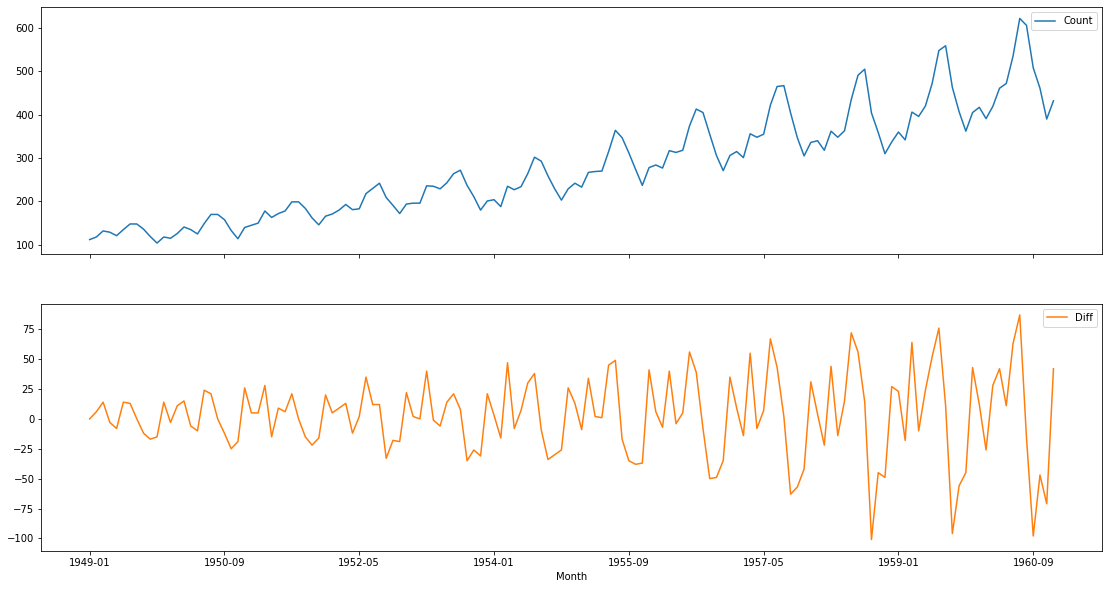
\includegraphics{main_files/figure-pdf/cell-7-output-2.png}

}

\end{figure}

\hypertarget{visual-inspection}{%
\subsection{Visual Inspection}\label{visual-inspection}}

At the first glance we see that the data does not contain missing
values. It's a discrete series, because we sample our values monthly. It
appears seasonal, which is in line with the meaning of the values in the
data frame - they reflect the number of air passengers, so it's natural
that we observe more passengers during, for example, summer.

\hypertarget{train-test-split}{%
\subsection{Train-Test Split}\label{train-test-split}}

There is no clear mention of the approach used to split the data into
training and test sets. Judging by the final forecast visualisation,
1958 appeared to be the cutoff point between training and test sets.
After this point there was an additional ARIMA curve until the end of
the series used to forecast air passenger volumes in comparison with the
actual time series.

We will therefore set 1949-1957 as the training set and 1958-1960 as the
test set.

\begin{Shaded}
\begin{Highlighting}[]
\NormalTok{data }\OperatorTok{=}\NormalTok{ data.reset\_index()}
\NormalTok{data[}\StringTok{\textquotesingle{}Date\textquotesingle{}}\NormalTok{] }\OperatorTok{=}\NormalTok{ data.}\BuiltInTok{apply}\NormalTok{(}\KeywordTok{lambda}\NormalTok{ x: datetime.datetime.strptime(x[}\StringTok{\textquotesingle{}Month\textquotesingle{}}\NormalTok{], }\StringTok{\textquotesingle{}\%Y{-}\%m\textquotesingle{}}\NormalTok{), axis }\OperatorTok{=} \DecValTok{1}\NormalTok{).dt.date}
\NormalTok{data }\OperatorTok{=}\NormalTok{ data.drop([}\StringTok{\textquotesingle{}Month\textquotesingle{}}\NormalTok{], axis }\OperatorTok{=} \DecValTok{1}\NormalTok{)}
\end{Highlighting}
\end{Shaded}

\begin{Shaded}
\begin{Highlighting}[]
\NormalTok{train }\OperatorTok{=}\NormalTok{ data.loc[data[}\StringTok{\textquotesingle{}Date\textquotesingle{}}\NormalTok{] }\OperatorTok{\textless{}}\NormalTok{ datetime.date(}\DecValTok{1958}\NormalTok{, }\DecValTok{1}\NormalTok{, }\DecValTok{1}\NormalTok{)]}
\NormalTok{train.tail()}
\end{Highlighting}
\end{Shaded}

\begin{longtable}[]{@{}llll@{}}
\toprule\noalign{}
& Count & Diff & Date \\
\midrule\noalign{}
\endhead
\bottomrule\noalign{}
\endlastfoot
103 & 467 & 2.0 & 1957-08-01 \\
104 & 404 & -63.0 & 1957-09-01 \\
105 & 347 & -57.0 & 1957-10-01 \\
106 & 305 & -42.0 & 1957-11-01 \\
107 & 336 & 31.0 & 1957-12-01 \\
\end{longtable}

\begin{Shaded}
\begin{Highlighting}[]
\NormalTok{test }\OperatorTok{=}\NormalTok{ data.loc[data[}\StringTok{\textquotesingle{}Date\textquotesingle{}}\NormalTok{] }\OperatorTok{\textgreater{}=}\NormalTok{ datetime.date(}\DecValTok{1958}\NormalTok{, }\DecValTok{1}\NormalTok{, }\DecValTok{1}\NormalTok{)]}
\NormalTok{test.head()}
\end{Highlighting}
\end{Shaded}

\begin{longtable}[]{@{}llll@{}}
\toprule\noalign{}
& Count & Diff & Date \\
\midrule\noalign{}
\endhead
\bottomrule\noalign{}
\endlastfoot
108 & 340 & 4.0 & 1958-01-01 \\
109 & 318 & -22.0 & 1958-02-01 \\
110 & 362 & 44.0 & 1958-03-01 \\
111 & 348 & -14.0 & 1958-04-01 \\
112 & 363 & 15.0 & 1958-05-01 \\
\end{longtable}

\hypertarget{stationarity}{%
\subsection{Stationarity}\label{stationarity}}

We should check if the series is stationary. As per visual inspection we
see that it should not be. We will use the \textbf{A}ugumented
\textbf{D}ickey-\textbf{F}uller (\textbf{ADF}) test
(\href{https://en.wikipedia.org/wiki/Augmented_Dickey\%E2\%80\%93Fuller_test}{\emph{Wikipedia}
link}), which is a part of the \texttt{statsmodels} library.

\begin{Shaded}
\begin{Highlighting}[]
\CommentTok{\# Small helper function for performing the DF test on a time series. }
\KeywordTok{def}\NormalTok{ ADF(series):}
\NormalTok{    (adf\_test, adf\_p) }\OperatorTok{=}\NormalTok{ sm.tsa.stattools.adfuller(series)[:}\DecValTok{2}\NormalTok{]}
    \BuiltInTok{print}\NormalTok{(}\SpecialStringTok{f"ADF Test Statistic = }\SpecialCharTok{\{}\NormalTok{adf\_test}\SpecialCharTok{\}}\SpecialStringTok{, p{-}value = }\SpecialCharTok{\{}\NormalTok{adf\_p}\SpecialCharTok{\}}\SpecialStringTok{"}\NormalTok{)}

\NormalTok{ADF(train[ }\StringTok{\textquotesingle{}Count\textquotesingle{}}\NormalTok{ ])}
\end{Highlighting}
\end{Shaded}

\begin{verbatim}
ADF Test Statistic = 1.0025865101330982, p-value = 0.9942931644042373
\end{verbatim}

Because the \emph{p-value} is outside the critical region, we
\textbf{fail to reject the null} hypothesis about the stationarity of
the series. This is in line with our initial expectations. We will
assume that the series is non-stationary.

The authors of the paper arrive at a different test statistic.

They actually obtain the following test statistic which assumes the use
of the entire time series (train + test).

\begin{Shaded}
\begin{Highlighting}[]
\CommentTok{\# Small helper function for performing the DF test on a time series. }
\KeywordTok{def}\NormalTok{ ADF(series):}
\NormalTok{    (adf\_test, adf\_p) }\OperatorTok{=}\NormalTok{ sm.tsa.stattools.adfuller(series)[:}\DecValTok{2}\NormalTok{]}
    \BuiltInTok{print}\NormalTok{(}\SpecialStringTok{f"ADF Test Statistic = }\SpecialCharTok{\{}\NormalTok{adf\_test}\SpecialCharTok{\}}\SpecialStringTok{, p{-}value = }\SpecialCharTok{\{}\NormalTok{adf\_p}\SpecialCharTok{\}}\SpecialStringTok{"}\NormalTok{)}

\NormalTok{ADF(data[ }\StringTok{\textquotesingle{}Count\textquotesingle{}}\NormalTok{ ])}
\end{Highlighting}
\end{Shaded}

\begin{verbatim}
ADF Test Statistic = 0.8153688792060482, p-value = 0.991880243437641
\end{verbatim}

For completeness, let's also check the stationarity of the series of
first differences:

\begin{Shaded}
\begin{Highlighting}[]
\NormalTok{ADF(train[ }\StringTok{\textquotesingle{}Diff\textquotesingle{}}\NormalTok{ ])}
\end{Highlighting}
\end{Shaded}

\begin{verbatim}
ADF Test Statistic = -2.349322039808016, p-value = 0.15655343854659332
\end{verbatim}

The p-value is still high enough for the null hypothesis not to be
rejected at 10\% confidence level.

\begin{Shaded}
\begin{Highlighting}[]
\NormalTok{ADF(data[ }\StringTok{\textquotesingle{}Diff\textquotesingle{}}\NormalTok{ ])}
\end{Highlighting}
\end{Shaded}

\begin{verbatim}
ADF Test Statistic = -2.889186069471266, p-value = 0.04662003920675332
\end{verbatim}

Extending the test to the entire series again, we \textbf{reject the
null} at the 95\% confidence level, better than the 0.07 p-value
reported by the authors. This indicates the first differences are
stationary and the the underlying series is I(1).

The authors of the paper describe that a \emph{logarithmic
transformation} is another useful option in removing the trend and
fluctuations in the series. Calculating the first difference was
sufficient though.

The steps that were taken by the authors include differencing and
removing seasonality. They \textbf{did not} mention how was the
seasonality removed - we can only guess here and perform our own
estimations.

With the process being classified as I(1), the authors proceeded to
determine the order of AR and MA models for the complete ARIMA model
using partial autocorrelation functions (PACF) and autocorrelation
functions (ACF), respectively.

\hypertarget{pacf-and-acf}{%
\subsection{PACF and ACF}\label{pacf-and-acf}}

Running PACF and ACF on the first differences on both training and
overall datasets is perfomed and depicted below. The shapes of both PACF
and ACF curves follow those produced by the authors with a closer match
for the training set. A similar set of lags are statistically
significant, as those in the paper.

\begin{Shaded}
\begin{Highlighting}[]
\KeywordTok{def}\NormalTok{ autocorr(data\_input, func\_type, ci):}
    \ControlFlowTok{if}\NormalTok{(func\_type }\OperatorTok{==} \StringTok{\textquotesingle{}PACF\textquotesingle{}}\NormalTok{):}
\NormalTok{        func\_data }\OperatorTok{=}\NormalTok{ sm.tsa.stattools.pacf(data\_input)}
    \ControlFlowTok{elif}\NormalTok{(func\_type }\OperatorTok{==} \StringTok{\textquotesingle{}ACF\textquotesingle{}}\NormalTok{):}
\NormalTok{        func\_data }\OperatorTok{=}\NormalTok{ sm.tsa.stattools.acf(data\_input)}
    
\NormalTok{    t }\OperatorTok{=} \BuiltInTok{len}\NormalTok{(data\_input)}
\NormalTok{    norminv }\OperatorTok{=}\NormalTok{ norm.ppf(ci }\OperatorTok{+}\NormalTok{ (}\DecValTok{1} \OperatorTok{{-}}\NormalTok{ ci) }\OperatorTok{/} \DecValTok{2}\NormalTok{)}
\NormalTok{    bound\_upper }\OperatorTok{=}\NormalTok{ norminv }\OperatorTok{/}\NormalTok{ t}\OperatorTok{**}\FloatTok{0.5}
\NormalTok{    bound\_lower }\OperatorTok{=} \OperatorTok{{-}}\NormalTok{ norminv }\OperatorTok{/}\NormalTok{ t}\OperatorTok{**}\FloatTok{0.5}
\NormalTok{    curve\_bound\_upper }\OperatorTok{=}\NormalTok{ [bound\_upper }\ControlFlowTok{for}\NormalTok{ i }\KeywordTok{in} \BuiltInTok{range}\NormalTok{(}\DecValTok{0}\NormalTok{,}\BuiltInTok{len}\NormalTok{(func\_data))]}
\NormalTok{    curve\_bound\_lower }\OperatorTok{=}\NormalTok{ [bound\_lower }\ControlFlowTok{for}\NormalTok{ i }\KeywordTok{in} \BuiltInTok{range}\NormalTok{(}\DecValTok{0}\NormalTok{,}\BuiltInTok{len}\NormalTok{(func\_data))]}
    
\NormalTok{    plt.plot(func\_data, label }\OperatorTok{=}\NormalTok{ func\_type)}
\NormalTok{    plt.plot(curve\_bound\_upper, }\StringTok{\textquotesingle{}k{-}{-}\textquotesingle{}}\NormalTok{, label }\OperatorTok{=} \StringTok{\textquotesingle{}Upper Bound\textquotesingle{}}\NormalTok{)}
\NormalTok{    plt.plot(curve\_bound\_lower, }\StringTok{\textquotesingle{}k{-}{-}\textquotesingle{}}\NormalTok{, label }\OperatorTok{=} \StringTok{\textquotesingle{}Lower Bound\textquotesingle{}}\NormalTok{)}
\NormalTok{    plt.title(func\_type)}
\NormalTok{    plt.show()}
\end{Highlighting}
\end{Shaded}

\begin{Shaded}
\begin{Highlighting}[]
\NormalTok{autocorr(data[ }\StringTok{\textquotesingle{}Diff\textquotesingle{}}\NormalTok{ ], }\StringTok{\textquotesingle{}PACF\textquotesingle{}}\NormalTok{, }\FloatTok{0.95}\NormalTok{)}
\end{Highlighting}
\end{Shaded}

\begin{figure}[H]

{\centering 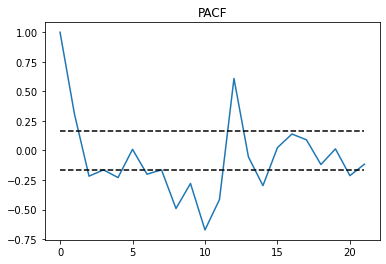
\includegraphics{main_files/figure-pdf/cell-16-output-1.png}

}

\end{figure}

\begin{Shaded}
\begin{Highlighting}[]
\NormalTok{autocorr(train[ }\StringTok{\textquotesingle{}Diff\textquotesingle{}}\NormalTok{ ], }\StringTok{\textquotesingle{}PACF\textquotesingle{}}\NormalTok{, }\FloatTok{0.95}\NormalTok{)}
\end{Highlighting}
\end{Shaded}

\begin{figure}[H]

{\centering 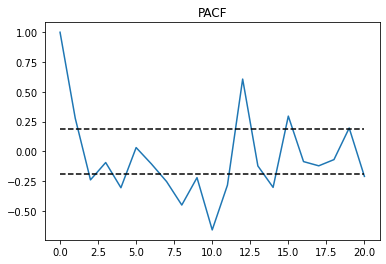
\includegraphics{main_files/figure-pdf/cell-17-output-1.png}

}

\end{figure}

\begin{Shaded}
\begin{Highlighting}[]
\NormalTok{autocorr(data[ }\StringTok{\textquotesingle{}Diff\textquotesingle{}}\NormalTok{ ], }\StringTok{\textquotesingle{}ACF\textquotesingle{}}\NormalTok{, }\FloatTok{0.95}\NormalTok{)}
\end{Highlighting}
\end{Shaded}

\begin{figure}[H]

{\centering 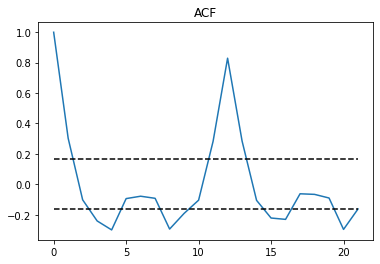
\includegraphics{main_files/figure-pdf/cell-18-output-1.png}

}

\end{figure}

\begin{Shaded}
\begin{Highlighting}[]
\NormalTok{autocorr(train[ }\StringTok{\textquotesingle{}Diff\textquotesingle{}}\NormalTok{ ], }\StringTok{\textquotesingle{}ACF\textquotesingle{}}\NormalTok{, }\FloatTok{0.95}\NormalTok{)}
\end{Highlighting}
\end{Shaded}

\begin{figure}[H]

{\centering 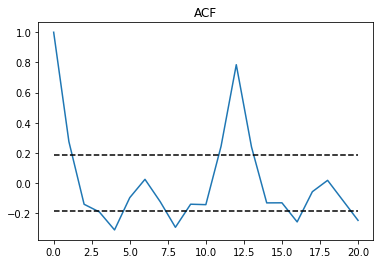
\includegraphics{main_files/figure-pdf/cell-19-output-1.png}

}

\end{figure}

There is some tendency to move towards zero over time in both PACF and
ACF, indicating AR and MA processes are likely to be able to explain the
underlying air passenger volume series. There are several spikes and
drops outside of the 95\% confidence interval bounds: using training
data, PACF visibly exceeds bounds at lags 8, 10 and 12 and ACF visibly
exceeds bounds at lags 4, 8 and 12. Therefore, it can be expected that
the components might follow p = 8/10/12 AR and q = 4/8/12 MA processes.

The authors of the paper, however, choose lower values for p and q,
ending up with an ARIMA(2,1,2) model. This is likely chosen in order to
maintain explainability and is supported by: - Maximum Likelihood
Estimation results which maximise the probability of obtaining the
observed data - Favourable AIC and BIC information criteria

\hypertarget{arima-model}{%
\subsection{ARIMA Model}\label{arima-model}}

With the ARIMA inputs determined, we can train the model and predict the
time series between 1958-1960.

\begin{Shaded}
\begin{Highlighting}[]
\KeywordTok{def}\NormalTok{ arima\_run(data\_input, order\_selection, print\_output, return\_model):}
\NormalTok{    arima\_out }\OperatorTok{=}\NormalTok{ ARIMA(data\_input, order}\OperatorTok{=}\NormalTok{order\_selection)}
\NormalTok{    arima\_out\_res }\OperatorTok{=}\NormalTok{ arima\_out.fit()}
    \ControlFlowTok{if}\NormalTok{ print\_output:}
        \BuiltInTok{print}\NormalTok{(arima\_out\_res.summary())}
        
\NormalTok{    arima\_out\_pred }\OperatorTok{=}\NormalTok{ arima\_out\_res.forecast(}\DecValTok{36}\NormalTok{)}
\NormalTok{    full }\OperatorTok{=}\NormalTok{ pd.concat([data\_input, arima\_out\_pred])    }
    \ControlFlowTok{if}\NormalTok{ print\_output:}
\NormalTok{        plt.plot(full)}
\NormalTok{        plt.title(}\StringTok{\textquotesingle{}ARIMA \textquotesingle{}} \OperatorTok{+} \BuiltInTok{str}\NormalTok{(order\_selection))}
\NormalTok{        plt.show()}
    
    \ControlFlowTok{if}\NormalTok{ return\_model:}
        \ControlFlowTok{return}\NormalTok{ full, arima\_out\_res}
    \ControlFlowTok{else}\NormalTok{:}
        \ControlFlowTok{return}\NormalTok{ full}
\end{Highlighting}
\end{Shaded}

\textbf{CALCULATE AIC AND BIC INFORMATION CRITERIA HERE}

\begin{Shaded}
\begin{Highlighting}[]
\NormalTok{full212, full212\_model }\OperatorTok{=}\NormalTok{ arima\_run(train[}\StringTok{\textquotesingle{}Diff\textquotesingle{}}\NormalTok{], (}\DecValTok{2}\NormalTok{,}\DecValTok{1}\NormalTok{,}\DecValTok{2}\NormalTok{), }\VariableTok{True}\NormalTok{, }\VariableTok{True}\NormalTok{)}
\end{Highlighting}
\end{Shaded}

\begin{verbatim}
                               SARIMAX Results                                
==============================================================================
Dep. Variable:                   Diff   No. Observations:                  108
Model:                 ARIMA(2, 1, 2)   Log Likelihood                -492.175
Date:                Fri, 16 Jun 2023   AIC                            994.351
Time:                        16:08:35   BIC                           1007.715
Sample:                             0   HQIC                           999.768
                                - 108                                         
Covariance Type:                  opg                                         
==============================================================================
                 coef    std err          z      P>|z|      [0.025      0.975]
------------------------------------------------------------------------------
ar.L1         -0.5080      0.128     -3.975      0.000      -0.758      -0.258
ar.L2          0.0939      0.100      0.939      0.347      -0.102       0.290
ma.L1         -0.0698     17.745     -0.004      0.997     -34.849      34.709
ma.L2         -0.9301     16.500     -0.056      0.955     -33.270      31.410
sigma2       553.6069   9844.942      0.056      0.955   -1.87e+04    1.98e+04
===================================================================================
Ljung-Box (L1) (Q):                   0.00   Jarque-Bera (JB):                 1.49
Prob(Q):                              0.95   Prob(JB):                         0.47
Heteroskedasticity (H):               4.69   Skew:                             0.09
Prob(H) (two-sided):                  0.00   Kurtosis:                         2.45
===================================================================================

Warnings:
[1] Covariance matrix calculated using the outer product of gradients (complex-step).
\end{verbatim}

\begin{figure}[H]

{\centering 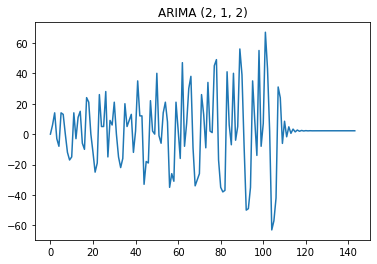
\includegraphics{main_files/figure-pdf/cell-21-output-2.png}

}

\end{figure}

\begin{Shaded}
\begin{Highlighting}[]
\NormalTok{full210, full210\_model }\OperatorTok{=}\NormalTok{ arima\_run(train[}\StringTok{\textquotesingle{}Diff\textquotesingle{}}\NormalTok{], (}\DecValTok{2}\NormalTok{,}\DecValTok{1}\NormalTok{,}\DecValTok{0}\NormalTok{), }\VariableTok{False}\NormalTok{, }\VariableTok{True}\NormalTok{)}
\end{Highlighting}
\end{Shaded}

\begin{Shaded}
\begin{Highlighting}[]
\NormalTok{full012, full012\_model }\OperatorTok{=}\NormalTok{ arima\_run(train[}\StringTok{\textquotesingle{}Diff\textquotesingle{}}\NormalTok{], (}\DecValTok{0}\NormalTok{,}\DecValTok{1}\NormalTok{,}\DecValTok{2}\NormalTok{), }\VariableTok{False}\NormalTok{, }\VariableTok{True}\NormalTok{)}
\end{Highlighting}
\end{Shaded}

\begin{Shaded}
\begin{Highlighting}[]
\NormalTok{full212\_series }\OperatorTok{=}\NormalTok{ []}
\NormalTok{val }\OperatorTok{=}\NormalTok{ data[}\StringTok{\textquotesingle{}Count\textquotesingle{}}\NormalTok{][}\DecValTok{0}\NormalTok{]}

\ControlFlowTok{for}\NormalTok{ i }\KeywordTok{in}\NormalTok{ full212:}
\NormalTok{    val }\OperatorTok{+=}\NormalTok{ i}
\NormalTok{    full212\_series.append(val)}
\end{Highlighting}
\end{Shaded}

\begin{Shaded}
\begin{Highlighting}[]
\NormalTok{plt.plot(data[}\StringTok{\textquotesingle{}Count\textquotesingle{}}\NormalTok{], label }\OperatorTok{=} \StringTok{\textquotesingle{}Observed\textquotesingle{}}\NormalTok{)}
\NormalTok{plt.plot(full212\_series, label }\OperatorTok{=} \StringTok{\textquotesingle{}Predicted\textquotesingle{}}\NormalTok{)}
\NormalTok{plt.title(}\StringTok{\textquotesingle{}Air Passenger Volume Assuming ARIMA(2,1,2)\textquotesingle{}}\NormalTok{)}
\NormalTok{plt.show()}
\end{Highlighting}
\end{Shaded}

\begin{figure}[H]

{\centering 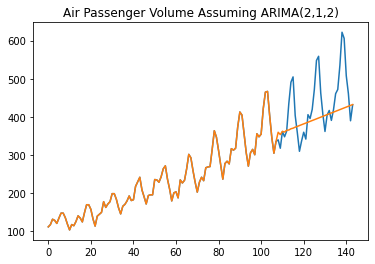
\includegraphics{main_files/figure-pdf/cell-25-output-1.png}

}

\end{figure}

Each of the ARIMAs chosen by the authors produced a poor fit in this
exercise. The least concerning out of the three models was ARIMA(2,1,2)
but still could not reproduce the visualised prediction in the paper.
Whilst it increased the series over time with the long-term trend
accurately, its variability diffused too quickly and it ignored the
seasonality.

\hypertarget{calculating-training-errors-and-comparison-with-rms-in-paper}{%
\subsubsection{Calculating training errors and comparison with RMS in
paper}\label{calculating-training-errors-and-comparison-with-rms-in-paper}}

Below we have calculated training errors similarly to ones calculated by
the authors of the original paper. As we can see, we were unable to
replicate the results using ARIMA model.

\begin{Shaded}
\begin{Highlighting}[]
\ControlFlowTok{for}\NormalTok{ model\_i }\KeywordTok{in}\NormalTok{ [}
\NormalTok{    (}\StringTok{"ARIMA (2,1,2)"}\NormalTok{, full212\_model, }\FloatTok{1.5023}\NormalTok{),}
\NormalTok{    (}\StringTok{"ARIMA (2,1,0)"}\NormalTok{, full210\_model, }\FloatTok{1.4721}\NormalTok{),}
\NormalTok{    (}\StringTok{"ARIMA (0,1,2)"}\NormalTok{, full012\_model, }\FloatTok{1.0292}\NormalTok{)}
\NormalTok{]:}
    \BuiltInTok{print}\NormalTok{(}\SpecialStringTok{f"}\SpecialCharTok{\{}\NormalTok{model\_i[}\DecValTok{0}\NormalTok{]}\SpecialCharTok{\}}\SpecialStringTok{: RMSE=}\SpecialCharTok{\{}\BuiltInTok{round}\NormalTok{(mean\_squared\_error(train[}\StringTok{\textquotesingle{}Diff\textquotesingle{}}\NormalTok{], model\_i[}\DecValTok{1}\NormalTok{].predict(), squared}\OperatorTok{=}\VariableTok{False}\NormalTok{),}\DecValTok{4}\NormalTok{)}\SpecialCharTok{\}}\SpecialStringTok{ (RMSE in paper = }\SpecialCharTok{\{}\NormalTok{model\_i[}\DecValTok{2}\NormalTok{]}\SpecialCharTok{\}}\SpecialStringTok{)"}\NormalTok{)}
    
\end{Highlighting}
\end{Shaded}

\begin{verbatim}
ARIMA (2,1,2): RMSE=23.6579 (RMSE in paper = 1.5023)
ARIMA (2,1,0): RMSE=28.6051 (RMSE in paper = 1.4721)
ARIMA (0,1,2): RMSE=24.3046 (RMSE in paper = 1.0292)
\end{verbatim}

In order to improve the forecast, more lags should be considered - these
were significant in the PACF and ACF after all. In addition, modifying
the functional form to a SARIMA model would better adapt to the data due
to the seasonality in air passenger volumes. We have expanded on the
paper by developing an alternative model which aims to reproduce the
forecast of the authors more accurately and produce significantly better
fit to the data.

\hypertarget{sarima}{%
\subsection{SARIMA}\label{sarima}}

Using SARIMA instead of ARIMA for forecasting the AirPassengers dataset
is better because SARIMA takes into account the seasonal patterns
present in the data. The AirPassengers dataset shows regular peaks and
troughs at specific intervals. SARIMA incorporates these seasonal
components, along with autoregressive and moving average components, to
capture the complex dynamics of the dataset more accurately. This
results in improved predictions, especially when dealing with data that
has clear seasonality like air passenger traffic. In summary, SARIMA is
a preferable choice over ARIMA for forecasting the AirPassengers dataset
due to its ability to handle seasonal patterns.

\hypertarget{time-series-decomposition}{%
\subsubsection{Time series
decomposition}\label{time-series-decomposition}}

\begin{Shaded}
\begin{Highlighting}[]
\NormalTok{result }\OperatorTok{=}\NormalTok{ seasonal\_decompose(data[}\StringTok{\textquotesingle{}Count\textquotesingle{}}\NormalTok{], period}\OperatorTok{=}\DecValTok{12}\NormalTok{, model}\OperatorTok{=}\StringTok{\textquotesingle{}additive\textquotesingle{}}\NormalTok{)}
\NormalTok{result.plot()}
\NormalTok{plt.show()}
\end{Highlighting}
\end{Shaded}

\begin{figure}[H]

{\centering 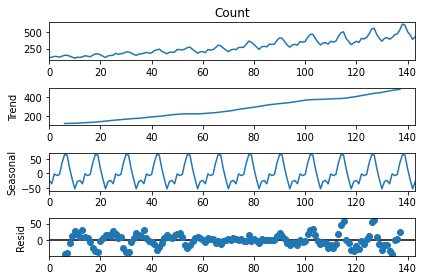
\includegraphics{main_files/figure-pdf/cell-27-output-1.png}

}

\end{figure}

Based on the plots above, we can observe that there are definitely
seasonal component. Hence, it would be a good idea to test SARIMA model
that probably would be able to replicate the paper's results.

Let's assume that authors forgot to describe that they use SARIMA model.
So, we will try the following SARIMA models: SARIMA (2,1,2)(0,1,0,12),
SARIMA (0,1,2)(0,1,0,12), SARIMA (2,1,0)(0,1,0,12).

\begin{Shaded}
\begin{Highlighting}[]
\KeywordTok{def}\NormalTok{ run\_sarima\_model(order,seasonal\_order, forecast\_horizon}\OperatorTok{=}\DecValTok{36}\NormalTok{, print\_summary}\OperatorTok{=}\VariableTok{False}\NormalTok{, print\_plot}\OperatorTok{=}\VariableTok{False}\NormalTok{):}
\NormalTok{    mod }\OperatorTok{=}\NormalTok{ sm.tsa.statespace.SARIMAX(data[}\StringTok{\textquotesingle{}Count\textquotesingle{}}\NormalTok{][:}\OperatorTok{{-}}\NormalTok{forecast\_horizon], trend}\OperatorTok{=}\StringTok{\textquotesingle{}c\textquotesingle{}}\NormalTok{, order}\OperatorTok{=}\NormalTok{order, seasonal\_order}\OperatorTok{=}\NormalTok{seasonal\_order)}
\NormalTok{    sarima\_model }\OperatorTok{=}\NormalTok{ mod.fit()}
    \ControlFlowTok{if}\NormalTok{ print\_summary:}
        \BuiltInTok{print}\NormalTok{(sarima\_model.summary())}

\NormalTok{    sarima\_pred }\OperatorTok{=}\NormalTok{ sarima\_model.forecast(forecast\_horizon)}
    
    \ControlFlowTok{if}\NormalTok{ print\_plot:}
\NormalTok{        plt.plot(data[}\StringTok{\textquotesingle{}Count\textquotesingle{}}\NormalTok{], label }\OperatorTok{=} \StringTok{\textquotesingle{}Observed\textquotesingle{}}\NormalTok{)}
\NormalTok{        plt.plot(pd.concat([data[}\StringTok{\textquotesingle{}Count\textquotesingle{}}\NormalTok{][:}\OperatorTok{{-}}\NormalTok{forecast\_horizon],sarima\_pred]), label }\OperatorTok{=} \StringTok{\textquotesingle{}Predicted\textquotesingle{}}\NormalTok{)}
\NormalTok{        plt.title(}\StringTok{\textquotesingle{}Air Passenger Volume\textquotesingle{}}\NormalTok{)}
\NormalTok{        plt.show()}
    
    \ControlFlowTok{return}\NormalTok{ sarima\_model, sarima\_pred}
\end{Highlighting}
\end{Shaded}

\begin{Shaded}
\begin{Highlighting}[]
\NormalTok{sarima212\_010\_12, sarima212\_010\_12\_pred }\OperatorTok{=}\NormalTok{ run\_sarima\_model((}\DecValTok{2}\NormalTok{,}\DecValTok{1}\NormalTok{,}\DecValTok{2}\NormalTok{), (}\DecValTok{0}\NormalTok{,}\DecValTok{1}\NormalTok{,}\DecValTok{0}\NormalTok{,}\DecValTok{12}\NormalTok{), print\_plot }\OperatorTok{=} \VariableTok{True}\NormalTok{)}
\end{Highlighting}
\end{Shaded}

\begin{figure}[H]

{\centering 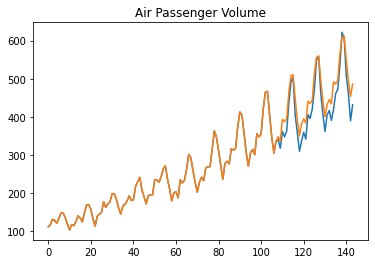
\includegraphics{main_files/figure-pdf/cell-29-output-1.png}

}

\end{figure}

\begin{Shaded}
\begin{Highlighting}[]
\NormalTok{sarima210\_110\_12, sarima210\_110\_12\_pred }\OperatorTok{=}\NormalTok{ run\_sarima\_model((}\DecValTok{2}\NormalTok{,}\DecValTok{1}\NormalTok{,}\DecValTok{0}\NormalTok{), (}\DecValTok{0}\NormalTok{,}\DecValTok{1}\NormalTok{,}\DecValTok{0}\NormalTok{,}\DecValTok{12}\NormalTok{), print\_plot }\OperatorTok{=} \VariableTok{True}\NormalTok{)}
\end{Highlighting}
\end{Shaded}

\begin{figure}[H]

{\centering 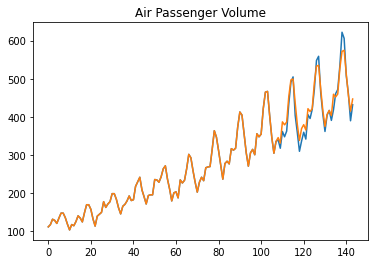
\includegraphics{main_files/figure-pdf/cell-30-output-1.png}

}

\end{figure}

\begin{Shaded}
\begin{Highlighting}[]
\NormalTok{sarima012\_110\_12, sarima012\_110\_12\_pred }\OperatorTok{=}\NormalTok{ run\_sarima\_model((}\DecValTok{0}\NormalTok{,}\DecValTok{1}\NormalTok{,}\DecValTok{2}\NormalTok{), (}\DecValTok{0}\NormalTok{,}\DecValTok{1}\NormalTok{,}\DecValTok{0}\NormalTok{,}\DecValTok{12}\NormalTok{), print\_plot }\OperatorTok{=} \VariableTok{True}\NormalTok{)}
\end{Highlighting}
\end{Shaded}

\begin{figure}[H]

{\centering 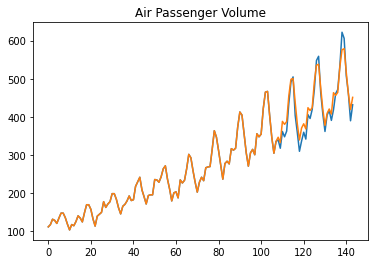
\includegraphics{main_files/figure-pdf/cell-31-output-1.png}

}

\end{figure}

As we can see, we managed to get predictions that take into account
seasonal component and it is getting us closer to replicating the
original results.

Let's calculate training errors again.

\begin{Shaded}
\begin{Highlighting}[]
\ControlFlowTok{for}\NormalTok{ model\_i }\KeywordTok{in}\NormalTok{ [}
\NormalTok{    (}\StringTok{"SARIMA (2,1,2) (0,1,0,12)"}\NormalTok{, sarima212\_010\_12, }\FloatTok{1.5023}\NormalTok{),}
\NormalTok{    (}\StringTok{"SARIMA (2,1,0) (0,1,0,12)"}\NormalTok{, sarima210\_110\_12, }\FloatTok{1.4721}\NormalTok{),}
\NormalTok{    (}\StringTok{"SARIMA (0,1,2) (0,1,0,12)"}\NormalTok{, sarima012\_110\_12, }\FloatTok{1.0292}\NormalTok{)}
\NormalTok{]:}
    \BuiltInTok{print}\NormalTok{(}\SpecialStringTok{f"}\SpecialCharTok{\{}\NormalTok{model\_i[}\DecValTok{0}\NormalTok{]}\SpecialCharTok{\}}\SpecialStringTok{: RMSE=}\SpecialCharTok{\{}\BuiltInTok{round}\NormalTok{(mean\_squared\_error(data[}\StringTok{\textquotesingle{}Count\textquotesingle{}}\NormalTok{][:}\OperatorTok{{-}}\DecValTok{36}\NormalTok{], model\_i[}\DecValTok{1}\NormalTok{].predict(), squared}\OperatorTok{=}\VariableTok{False}\NormalTok{),}\DecValTok{4}\NormalTok{)}\SpecialCharTok{\}}\SpecialStringTok{ (RMSE in paper = }\SpecialCharTok{\{}\NormalTok{model\_i[}\DecValTok{2}\NormalTok{]}\SpecialCharTok{\}}\SpecialStringTok{)"}\NormalTok{)}
    
\end{Highlighting}
\end{Shaded}

\begin{verbatim}
SARIMA (2,1,2) (0,1,0,12): RMSE=15.379 (RMSE in paper = 1.5023)
SARIMA (2,1,0) (0,1,0,12): RMSE=15.6072 (RMSE in paper = 1.4721)
SARIMA (0,1,2) (0,1,0,12): RMSE=15.625 (RMSE in paper = 1.0292)
\end{verbatim}

Comparing to ARIMA models, we got much lower RMSE metric for SARIMA
models. Unfortunately, we are still too far from the results presented
in the paper.



\end{document}
